\documentclass[justified, openany]{tufte-book}

\usepackage[utf8]{inputenc}
\usepackage[english]{babel}
\usepackage{blindtext}
\usepackage{todonotes}

\setcounter{secnumdepth}{1}
\setcounter{tocdepth}{1}

% turn on numbering for parts and chapters

\usepackage{amsthm, amsmath, amssymb}
\usepackage{setspace, graphicx, enumerate}

\usepackage{stmaryrd}

% For nicely typeset tabular material
\usepackage{booktabs}

\usepackage{listings}
\lstloadlanguages{Haskell}

\usepackage{permute}

\newcommand{\monthyear}{%
  \ifcase\month\or January\or February\or March\or April\or May\or June\or
  July\or August\or September\or October\or November\or
  December\fi\space\number\year
}

% For graphics / images
\usepackage{graphicx}
\usepackage{fancyvrb}
\fvset{fontsize=\normalsize}
\usepackage{xspace}

\usepackage{pgf, tikz}
\usetikzlibrary{arrows,automata,decorations.pathmorphing,backgrounds,positioning,fit,petri,shapes.geometric,calc}

\usepackage{units}

\usepackage{bibentry}

\usepackage{tcolorbox}

\usepackage{enumitem}

\usepackage{bm}

\usepackage{mmacells}

\usepackage{oplotsymbl}

\usepackage{pdfpages}

\usepackage[nottoc]{tocbibind}

\theoremstyle{plain}% default 
\newtheorem{thm}{Theorem}[chapter] 
\newtheorem{lem}[thm]{Lemma} 
\newtheorem{prop}[thm]{Proposition} 
\newtheorem*{cor}{Corollary} 

\theoremstyle{definition} 
\newtheorem{defn}[thm]{Definition}
\newtheorem{conj}[thm]{Conjecture}
\newtheorem{exmp}[thm]{Example}
\newtheorem{exer}[thm]{Exercise}

\newtheorem{proofpart}{Proof Part}[thm]

\theoremstyle{remark} 
\newtheorem*{rem}{Remark} 
\newtheorem*{note}{Note} 
\newtheorem{case}{Case}
\newtheorem{thminv}{Invariant}[chapter] 


\newtcolorbox{problem}{title={Problem}}

\newenvironment{dedication}
    {\vspace{6ex}\begin{quotation}\begin{center}\begin{em}\begin{large}}
    {\par\end{large}\end{em}\end{center}\end{quotation}}

\mmaDefineMathReplacement[≤]{<=}{\leq}
\mmaDefineMathReplacement[≥]{>=}{\geq}
\mmaDefineMathReplacement[≠]{!=}{\neq}
\mmaDefineMathReplacement[→]{->}{\to}[2]
\mmaDefineMathReplacement[⧴]{:>}{:\hspace{-.2em}\to}[2]
\mmaDefineMathReplacement{∉}{\notin}
\mmaDefineMathReplacement{∞}{\infty}
\mmaDefineMathReplacement{𝕕}{\mathbbm{d}}


\mmaSet{
  morefv={gobble=2},
  linklocaluri=mma/symbol/definition:#1,
  morecellgraphics={yoffset=1.9ex}
}



\title{Math notes - Devil's chessboard}
\author{Uwe Hoffmann}
\hypersetup{colorlinks, pdftitle={Math notes - Devil's chessboard}}

\begin{document}

\setcounter{chapter}{1}
\section*{Devil's chessboard}

\newthought{Hamming codes} are used to solve the problem\footnote{\bibentry{devils_chessboard}} in this note.

You, your friend, and the Devil play a game. You and the Devil are in the room with a chess board with $64$ tokens on it, one on each square. Meanwhile, your friend is outside of the room. The token can either be on an up position or a down position, and the difference in position is distinguishable to the eye. The Devil mixes up the positions (up or down) of the tokens on the board and chooses one of the  squares and calls it the magic square. Next, you may choose one token on a square and flip its position. Then, your friend comes in and must guess what the magic square was by looking on the squares on the board.\footnote{
Details:
\\
\begin{enumerate}
\item You \textbf{may} flip a token. As in, you are not forced to flip a token; you may choose to not flip a token.

\item You can't just tell your friend what square it is. Or point to it. Or text him it. Or... you get the point.

\item Your friend knows the strategy as well (you tell him beforehand).

\item If you don't get it right, the Devil takes your soul. High stakes.
\end{enumerate}}

\vspace{10 mm}
\begin{problem}
Show that there is a winning strategy such that your friend can always know what square the magic square is.
\end{problem}

\begin{marginfigure}[0.0in]

\includegraphics[scale=0.5]{Richard_Hamming.jpg}
\end{marginfigure}

There might be solutions that exploit the chessboard geometry with its black and white fields. We will ignore the chessboard angle though and use this problem as an excuse to dive into the topic of linear codes. We will solve the problem by treating the token information as a 64-bit word and we will devise a winning strategy that involves a Hamming\footnote{Richard Hamming was one of the founders of modern coding theory. \url{http://en.wikipedia.org/wiki/Richard_Hamming}} code (a type of perfect linear code).

But first lets introduce linear codes\index{linear code}. We operate in the field $\mathbb{F}_q$ of integers modulo a prime $q$. 

\begin{defn}\label{linearCodeDef}
A \textbf{linear code} $C$ of words of length $n$ is a subspace of the vector space $\mathbb{F}^n_q$. Let $\dim C = k$, then we say that $C$ is a $[n, k]_q$ linear code.
\end{defn}

Given a basis $\{\bm{c_1}, \bm{c_2}, \ldots, \bm{c_k}\}$ of $C$, we can build a matrix $G \in \mathbb{F}_q^{k \times n}$ using the $\bm{c_i}$ basis vectors as rows. Then $C$ is the row space of $G$ and $G$ is called a \textbf{generator matrix}\index{generator matrix} of $C$. We have\footnote{We treat vectors as row vectors in this section. That means that $\bm{x} \in \mathbb{F}_q^k$ is a matrix $\mathbb{F}_q^{1 \times k}$.}

$$
C = \{\bm{x} G: \bm{x} \in \mathbb{F}_q^k\},
$$

\noindent so a code $C$ is made from all linear combinations of the row vectors of its generator matrix.

Let $G'$ be the row reduced echelon form of $G$. By definition $G$ has full row rank, so $G'$ has only nonzero rows. If 
$
G' = \left[\begin{smallmatrix}
I_k & | & A_{k \times (n - k)}
\end{smallmatrix}\right]
$ 
for identity matrix $I_k$ and some matrix $A$ then the generator matrix $G'$ is in \textbf{standard form}\footnote{Not every generator matrix can be row reduced to the standard form. For example 
$$
\begin{bmatrix}
1 & 1 & 0 & 0 \\
0 & 0 & 1 & 1 
\end{bmatrix}
$$
cannot.}. Row operations preserve the row space, so $G'$ also generates $C$.

\begin{defn}\label{parityCheckDef}
Given a $[n, k]_q$ linear code $C$, matrix $H \in \mathbb{F}_q^{(n-k) \times n}$ is a \textbf{parity check matrix}\index{parity check matrix} for $C$, if $C = nullspace(H)=\{\bm{c} \in \mathbb{F}_q^n: H \bm{c}^T = 0\}$.
\end{defn}

\begin{thm}\label{generatorParityCheckRel}
Given a $[n, k]_q$ linear code $C$ and a generator matrix $
G = \left[\begin{smallmatrix}
I_k & | & A_{k \times (n - k)}
\end{smallmatrix}\right]
$ for $C$ in standard form, then $
H = \left[\begin{smallmatrix}
-A^T_{(n - k) \times k} & | & I_{n - k}
\end{smallmatrix}\right]
$ is a parity check matrix\footnote{With $G$ in standard form this theorem let's us construct a parity check matrix very easily. Also worth noting that in standard form we generate a code word from a message $\bm{x} \in \mathbb{F}_q^k$ by appending $n - k$ parity check bits to the message with $\bm{x} G$. We check if the transmitted and received word $\bm{y} \in \mathbb{F}_q^n$ is a valid code word by verifying $H \bm{y}^T = 0$. If true then the first k positions of $\bm{y}$ are the original message $\bm{x}$.} for $C$.
\end{thm}

\begin{proof}

Let $\bm{c} \in C$ be a code word from $C$. Then there exists an $\bm{x} \in \mathbb{F}_q^k$ such that $\bm{c} = \bm{x} G$.
We have

\begin{align*}
 H \bm{c}^T &= H (\bm{x} G)^T \\
        &= \left[ -A^T_{(n - k) \times k} | I_{n - k} \right] \left(\bm{x} \left[ I_k | A_{k \times (n - k)} \right]\right)^T \\
        &=  \left[ -A^T_{(n - k) \times k} | I_{n - k} \right] \left[ \begin{array}{c}
                                                                           I_k \\ \hline
                                                                           A^T_{(n - k) \times k}
                                                                       \end{array}  \right] \bm{x}^T \\
        &= (-A^T + A^T) \bm{x}^T \\
        &= 0
\end{align*}

This means that $C \subseteq nullspace(H)$. We have $\dim C = k$ and 
$$
\dim nullspace(H) = n - rank(H) = n - n + k = k,
$$
so $C = nullspace(H)$ and $H$ is a parity check matrix for $C$.

\end{proof}

What can we do if the generator matrix is not in standard form? Swapping columns in the generator matrix does not preserve the row space, so the linear code generated with the modified matrix is clearly not the same as the original code, but it is an equivalent code\footnote{A $[n, k_1]_q$ linear code $C_1$ is equivalent to a $[n, k_2]_q$ linear code $C_2$ if there is a permutation $\pi \in S_n$ such that when $\pi$ is applied to the coordinate indices of all the code words from $C_1$, it produces all the code words from $C_2$. Equivalent linear codes have the same dimension $k_1=k_2$.}. 

\begin{defn}\label{hammingDistDef}
The \textbf{Hamming distance}\index{Hamming distance} $d(\bm{x}, \bm{y})$ between two vectors $\bm{x}, \bm{y} \in \mathbb{F}_q^n$ is the number of positions in which the vectors differ. With $\bm{x} = x_1 x_2 \ldots x_n$ and $\bm{y} = y_1 y_2 \ldots y_n$ we have
$$
d(\bm{x}, \bm{y}) = |\{i : 1 \leq i \leq n : x_i \neq y_i\}|
$$
The \textbf{Hamming weight}\index{Hamming weight} $w(\bm{x})$ is the number of positions that differ from zero:
$$
w(\bm{x}) = |\{i : 1 \leq i \leq n : x_i \neq 0\}| = d(\bm{x}, \bm{0})
$$
\end{defn}

We will use the following properties of Hamming distances:

\marginnote{\textit{Proof} of Lemma \ref{hammingtriangle} \\
The first three properties are obvious from the definition of Hamming distance. For the last property let $i$ be an index where $\bm{x}$ and $\bm{y}$ differ, so $x_i \neq y_i$. For vector $\bm{z}$ we can have the following cases for position $i$:
\begin{align*}
& z_i = x_i \Rightarrow z_i \neq y_i \\
& z_i = y_i \Rightarrow z_i \neq x_i \\
& z_i \neq x_i \land z_i \neq y_i
\end{align*}
In each of these cases the contribution of $z_i$ to $d(\bm{x}, \bm{z}) + d(\bm{z}, \bm{y})$ is at least one, whereas on the left side position $i$ contributes one to $d(\bm{x}, \bm{y})$. A similar analysis holds for indices $i$ where $x_i=y_i$.
\qed}

\begin{lem}\label{hammingtriangle}
\begin{align*}
&\forall \bm{x}, \bm{y} \in \mathbb{F}_q^n : d(\bm{x}, \bm{x}) \geq 0 \\
&\forall \bm{x}, \bm{y} \in \mathbb{F}_q^n : d(\bm{x}, \bm{y}) = 0 \Leftrightarrow x = y \\
&\forall \bm{x}, \bm{y} \in \mathbb{F}_q^n : d(\bm{x}, \bm{y}) = d(\bm{y}, \bm{x}) \\
&\forall \bm{x}, \bm{y}, \bm{z} \in \mathbb{F}_q^n : d(\bm{x}, \bm{y}) \leq d(\bm{x}, \bm{z}) + d(\bm{z}, \bm{y})
\end{align*}
\end{lem}

\begin{defn}\label{hammingDistCodeDef}
The \textbf{minimum distance} of $C$ is:
$$
d(C) = \min \{d(\bm{x}, \bm{x'}) : \bm{x}, \bm{x'} \in C \land \bm{x} \neq \bm{x'} \} = \min \{w(\bm{x}) : \bm{x} \in C \}
$$
\end{defn}

The minimum distance\index{minimum distance} is important enough that we add it to the characteristic notation of a linear code: $[n, k, d]_q$ is a linear  code over field $\mathbb{F}_q$ with bit strings of length $n$, code dimension $k$ and minimum distance between code words $d$.

The next lemma establishes a connection between the minimum distance of a linear code and one of its parity check matrix.

\begin{lem}\label{minCodeParityCheckRel}
The minimum distance of a code $C$ equals the minimum number of linearly dependent columns in one of its parity check matrices. 
\end{lem}

\marginnote{\textit{Proof} of Lemma \ref{minCodeParityCheckRel} \\
Let $H$ be a parity check matrix of $[n, k, d]_q$ linear code $C$. There must be a code word $\bm{c}$ with $w(\bm{c}) = d$.
$\bm{c}$ belongs to the nullspace of $H$, so

$$
H \bm{c}^T = \bm{0}
$$

But $H \bm{c}^T$ is a linear combination of column vectors of $H$, with $d$  nonzero coefficients, so the column vectors in this linear combination are linearly dependent. 
\qed}

So far we have worked with fields $\mathbb{F}_q$ of any prime $q$. Now we switch to the binary world $q=2$ and $\mathbb{F}_2$. Our vectors are bit strings. We transmit these bit strings over a binary symmetric channel. 

\begin{defn}\label{symChanDef}
In a \textbf{binary symmetric channel}\index{binary symmetric channel} each bit sent has the same probability $p < \frac{1}{2}$ of being received incorrectly.
\end{defn}

We send a code word $\bm{x} \in C$ from a $[n, k]_2$ linear code $C$ over a binary symmetric channel and receive a bit string $\bm{y}$. If there were no transmission errors, then $y=x$. If there were errors, we want to find the most likely code word $\bm{x}$ that was transmitted given the errors in $\bm{y}$.

One decoding strategy\footnote{Finding an appropriate code word for the transmitted bit string is called \textit{decoding}. Finding the most likely code word is called \textit{maximum likelihood decoding}.} would be to choose a code word $\bm{x}$ with minimum Hamming distance over all code words from $C$ to received bit string $\bm{y}$. This type of decoding is called \textit{nearest neighbor decoding}. The chosen $\bm{x}$ is not always unique.

\begin{thm}\label{nnDmaximumLike}
In a binary symmetric channel with error probability $p < \frac{1}{2}$ the nearest neighbor decoding is a maximum likelihood decoding.
\end{thm}

\begin{proof}
Given a bit string $\bm{y} \in \mathbb{F}_2^n$ received through the channel, let $P_{\bm{y}}(\bm{x})$ be the probability that the code word $\bm{x}$ was sent when $\bm{y}$ was received. Because the channel is a binary symmetric channel, we have

$$
P_{\bm{y}}(\bm{x}) = p^{d(\bm{x}, \bm{y})} (1 - p)^{n - d(\bm{x}, \bm{y})}
$$

Consider two code words $\bm{x}$ and $\bm{x'}$ such that $d(\bm{x}, \bm{y}) \leq d(\bm{x'}, \bm{y})$. Because $p < \frac{1}{2}$, we then have $P_{\bm{y}}(\bm{x}) \geq P_{\bm{y}}(\bm{x'})$. It follows that
$$
\max_{\bm{x} \in C} P_{\bm{y}}(\bm{x}) = \min_{\bm{x} \in C} d(\bm{x}, \bm{y})
$$
so the likeliest code word is the nearest neighbor to $\bm{y}$.
\end{proof}

For the rest of this section we use nearest neighbor decoding. We want to know if we can detect and possibly correct a transmission with errors. Let's define clearly what we mean by that. A transmission is a pair $(\bm{x}, \bm{y}) \in C \times \mathbb{F}_2^n$, where a code word $\bm{x}$ was sent and a bit strings $\bm{y}$ was received. It has $d(\bm{x}, \bm{y})$ transmission errors. The nearest neighbor decoding $nnd(\bm{y})$ finds a code word (not necessarily unique) closest to $\bm{y}$. The following holds by definition:

$$
d(\bm{y}, nnd(\bm{y})) = \min_{\bm{c} \in C} d(\bm{y}, \bm{c})
$$

If no errors occurred in the transmission, then $\bm{x} = \bm{y}$ and also $d(\bm{x}, \bm{y}) = 0$ and $nnd(\bm{y}) = \bm{x}$. If errors in the transmission occurred we want to:

\begin{enumerate}[label=\textbf{E.\arabic*}]
\item \label{transmissionErrorRecogOne} detect that errors happened, i.e. establish that $\bm{y} \notin C$.
\item \label{transmissionErrorRecogTwo} correct the errors, i.e. establish $nnd(\bm{y}) = \bm{x}$.
\end{enumerate}

The next theorem describes the conditions for \ref{transmissionErrorRecogOne}.

\begin{thm}\label{linearCodeDetectErrors}
Given a $[n, k, d]_2$ linear binary code $C$, we can detect that any transmission with up to $e$ errors was erroneous if and only if $d > e$.
\end{thm}

\begin{proof}

\noindent$(\Rightarrow)$ Let $(\bm{x}, \bm{y})$ be a transmission with $d(\bm{x}, \bm{y}) \leq e < d$ errors. Assume $\bm{y} \in C$. Then $d(\bm{x}, \bm{y}) \leq e < d$ is a contradiction to $d$ being the minimal distance of $C$. It follows that $\bm{y} \notin C$.

\noindent$(\Leftarrow)$ We can detect that any transmission with up to $e$ errors was erroneous. Assume $d \leq e$. Then there exist two code words $\bm{x} \neq \bm{x'}$ such that $d(\bm{x}, \bm{x'}) \leq e$. Now consider transmission $(\bm{x}, \bm{x'})$. It's impossible to detect that it had errors because $\bm{x'}$ is a code word. This is a contradiction with the fact that we can detect that any transmission with up to $e$ errors was erroneous. So $d > e$.
\end{proof}

\begin{marginfigure}[0.5in]
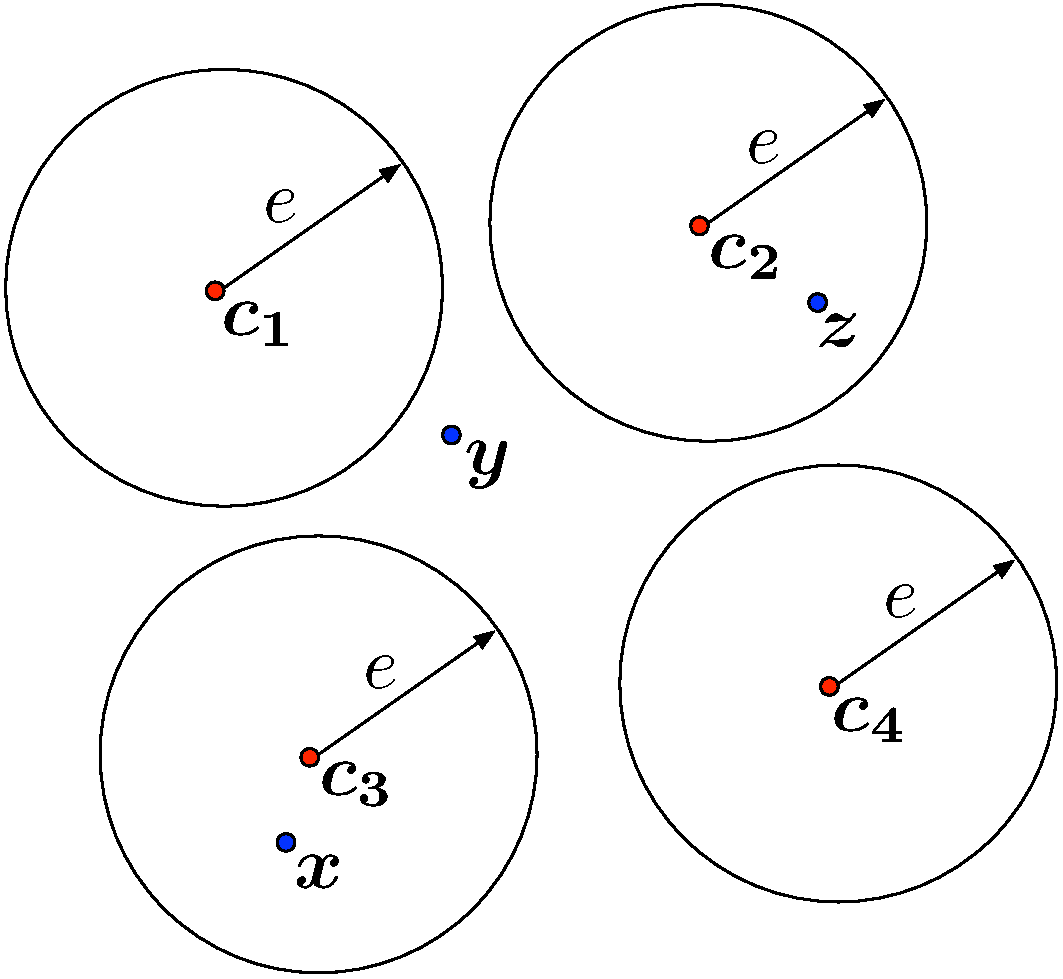
\includegraphics[scale=0.3]{hammingSpheres.pdf}
\caption{A Hamming sphere for code word $\bm{c}$ with radius  $e$ is the set \\
$\{\bm{x}: d(\bm{x}, \bm{c}) \leq e\}$. In this figure the spheres don't overlap, so vectors (blue dots) that fall within a sphere can be error-corrected to code words (red dots).}
\label{fig:hammingSpheres}
\end{marginfigure}

For \ref{transmissionErrorRecogTwo} we have this theorem:

\begin{thm}\label{linearCodeCorrectErrors}
Given a $[n, k, d]_2$ linear binary code $C$, we can correct any transmission with up to $e$ errors if $d > 2 e$.
\end{thm}

\begin{proof}
Let $(\bm{x}, \bm{y})$ be a transmission with $d(\bm{x}, \bm{y}) \leq e$ errors and $d > 2 e$. Assume $nnd(\bm{y}) \neq \bm{x}$. Then $d(\bm{y}, nnd(\bm{y})) \leq e$ (otherwise $\bm{x}$ would be closer than $nnd(\bm{y})$ to $\bm{y}$). We have
$$
d(\bm{x}, nnd(\bm{y})) \leq d(\bm{x}, \bm{y}) + d(\bm{y}, nnd(\bm{y})) \leq e + e = 2 e
$$
which contradicts $d > 2 e$. So $nnd(\bm{y}) = \bm{x}$.

\end{proof}

Theorems \ref{linearCodeDetectErrors} and \ref{linearCodeCorrectErrors} tell us that a large minimum distance $d(C)$ allows us to detect and correct more errors. But a large minimum distance between code words also limits the number of code words. The following theorem puts an upper bound on the number of code words given a minimum distance.

\begin{thm}\label{hammingBound}
Given a $[n, k, 2 t + 1]_2$ linear binary code $C$, we have
$$
|C| \leq \frac{2^n}{\sum_{i = 0}^t \binom{n}{i}}
$$
This upper bound is called \textbf{Hamming bound}\index{Hamming bound}.
\end{thm}

\begin{proof}

Given a bit string $\bm{x}$ and an integer $i \leq n$, there are $\binom{n}{i}$ ways to choose the $i$ positions at which $\bm{x}$ and and another bit string $\bm{y}$ differ. So there are $\binom{n}{i}$ bit strings $\bm{y}$ with $d(\bm{x}, \bm{y}) = i$. This means there are 
$$
\sum_{i = 0}^t \binom{n}{i}
$$
bit strings $\bm{y}$ with $d(\bm{x}, \bm{y}) \leq t$.

On the other hand, a bit string $\bm{y}$ with $d(\bm{y}, \bm{x}) \leq t$ to a code word $\bm{x}$ cannot have the same  
$d(\bm{y}, \bm{x'}) \leq t$ to a different code word $\bm{x'}$ because then

$$
d(\bm{x}, \bm{x'}) \leq d(\bm{x}, \bm{y}) + d(\bm{y}, \bm{x'}) \leq t + t \leq 2 t
$$

which is a contradiction to $d(C) = 2 t + 1$.

So for each code word, we have at most $\sum_{i = 0}^t \binom{n}{i}$ bit strings with Hamming distance $\leq t$ and we cannot have the same bit strings near two different code words. We have $2^n$ bit strings, so

$$
|C| \sum_{i = 0}^t \binom{n}{i} \leq 2^n
$$

\end{proof}

A binary linear code that achieves equality in the Hamming bound \ref{hammingBound} is called a \textbf{perfect code}\index{perfect code}.

We are now ready to define Hamming codes\index{Hamming code}.

\begin{defn}\label{hammingCode}
A Hamming code $\mathfrak{H}_r$ of order $r$ (where $r$ is a positive integer) is a binary linear code with the parity check matrix
with columns that are all the $2^r - 1$ nonzero bit strings of length $r$.
\end{defn}

Changing the order of the columns in the parity check matrix produces equivalent codes with the same minimum distance. So for easier analysis we now consider Hamming codes with parity check matrix in standard form, ie the last $r$ columns form the identity matrix $I_r$, so $
H = \left[\begin{smallmatrix}
A_{r \times (n - r)} & | & I_{r}
\end{smallmatrix}\right]
$, with $n = 2^r - 1$. From theorem \ref{generatorParityCheckRel} we then know the generator matrix is $
G = \left[\begin{smallmatrix}
I_{n - r} & | & -A_{(n - r) \times r}^T
\end{smallmatrix}\right] = \left[\begin{smallmatrix}
I_{n - r} & | & A_{(n - r) \times r}^T
\end{smallmatrix}\right]
$, since we operate in $\mathbb{F}_2$. We can see that $\dim \mathfrak{H}_r = n - r$. What is the minimum distance of $\mathfrak{H}_r$? All columns are nonzero and distinct, so no two columns are linearly dependent\footnote{Again, this is in $\mathbb{F}_2$. The sum of two distinct columns is always nonzero, so a linear combination that is zero has to have coefficients zero, hence linearly independent.}. But consider the linear combination of the three columns 
$$
[1, 1, 0, \ldots, 0]^T + [1, 0, 0, \ldots, 0]^T + [0, 1, 0, \ldots, 0]^T = \bm{0}^T
$$
They are linearly dependent. From lemma \ref{minCodeParityCheckRel} it follows that $d(\mathfrak{H}_r) = 3$, so $\mathfrak{H}_r$ is a $[2^r - 1, 2^r - 1 - r, 3]_2$ binary linear code. According to theorem \ref{linearCodeCorrectErrors} it can correct transmissions with one error. 

\begin{thm}\label{hammingPerfect}
$\mathfrak{H}_r$ is a perfect code.
\end{thm}

\begin{proof}

The generator matrix has full row rank, so we need all linear combinations of the rows to get all the code words. This are binary words, so there are $2^{n - r}$ distinct linear combinations. It means $|\mathfrak{H}_r| = 2^{n - r}$.

Inserting into formula of theorem \ref{hammingBound}, we get\footnote{With $t = 1$, because $d(\mathfrak{H}_r) = 3$.}

$$
2^{n - r} \sum_{i = 0}^1 \binom{n}{i} = 2^{n - r} (1 + n) = 2^{n - r} (1 + 2^r - 1) = 2^{n - r} 2^r = 2^n
$$

\end{proof}

This concludes our dive into linear codes and Hamming codes. Let's return to our problem and solve it using Hamming codes. The state of the chessboard is a binary word of length $64$. We use $r = 6$, so Hamming code $\mathfrak{H}_6$. The word length is $2^6 - 1 = 63$. We agree that the devil choosing bit $64$ is a special case which we handle later. For now imagine the chessboard as a $63$-bit binary word and the devil only choosing a magic field between $1$ and $63$.

The winning strategy can be summarized as follows: the first player needs to modify the $63$-bit word (by flipping at most one bit) in such a way that the magic field is the one bit error of a code word in $\mathfrak{H}_6$. Then the second player only has to come in, decode the modified chessboard and point to the corrected error which is the same magic field\footnote{Decoding\label{decodingSideNote} is done as follows: $\bm{x}$ needs to be decoded. It is one bit away from a code word $\bm{c}$ with error at bit $k$. Let $\bm{e_k}$ be the unit vector with bit $k$ set. So $\bm{x} = \bm{c} + \bm{e_k}$ and 
$$
H \bm{x} = H (\bm{c} + \bm{e_k}) = H \bm{e_k}
$$
Since $\bm{e_k}$ is be the unit vector with bit $k$ set, $H \bm{e_k}$ is column $k$ from the parity check matrix $H$. To decode we calculate $H \bm{x}$ and look to see which column in $H$ the result is. To save the lookup step we can be even more elegant. Instead of the parity check matrix in standard form, we choose a parity check matrix where column $k$ is the bit representation of $k$. Instead of lookup we just reverse the bit representation back to the integer $k$.
}.

Is this always possible? We know that Hamming codes are perfect codes, so any $63$-bit word is at most one bit away from a code word. We have the following cases for the initial state of the chessboard:

\begin{itemize}
\item  It happens to be a code word in $\mathfrak{H}_6$. Then the first player flips the magic field bit, producing an error there.

\item It happens to be a $63$-bit word that is a one bit error at the magic field. The first player doesn't flip any bit in this case.

\item It happens to be a $63$-bit word with a one bit error different from the magic field.
\end{itemize}

The last case needs a little thinking. Assume $H$ is the parity check matrix for our $\mathfrak{H}_6$ Hamming code and assume the state of the chessboard is $\bm{x}$, which is one bit error from a code word $\bm{c_1}$. Also let $1 \leq m \leq 63$ be the magic field bit and $\bm{e_m}$ the unit vector with bit $m$ set. The one bit error is different from the magic field, so $\bm{x} - \bm{c_1} \neq \bm{e_m}$. Let $\bm{y} = \bm{x} - \bm{e_m}$, which is also one bit away from a code word $\bm{c_2}$, with error bit $k$. So 
$\bm{y} = \bm{c_2} + \bm{e_k}$.

Now consider $\bm{x} - \bm{e_k}$:
$$
H (\bm{x} - \bm{e_k}) = H (\bm{y} + \bm{e_m} - \bm{e_k}) = H (\bm{y} - \bm{e_k}) + H \bm{e_m} = H \bm{c_2} + H \bm{e_m} = H \bm{e_m}
$$

So $\bm{x} - \bm{e_k}$ has one bit error at the magic field, which is what we want. Flipping bit $k$ on the initial chessboard $\bm{x}$ achieves that.

In all three cases the modified chessboard is one bit away from a code word with the error at the magic field and the chessboard was modified by flipping at most one bit. The players agree that if the chessboard is a code word instead, then the devil chose bit $64$ as the magic field, which handles the special case. Modifying the chessboard to get a code word can also be done by flipping at most one bit. This scales to any chessboard with size a power of two.

\begin{fullwidth}

What follows is a Mathematica session illustrating the strategy. We use a parity check matrix with column $k$ the bit representation of integer $k$. This simplifies decoding as remarked in the side note \ref{decodingSideNote} above.

The function \textit{hamming} generates the parity check matrix for a Hamming code with a given $r$.

\begin{mmaCell}[morefunctionlocal={i},morepattern={r, r_Integer}]{Code}
  hamming[r_Integer] := Transpose[Table[IntegerDigits[i, 2, r], {i, 1, 2^r - 1}]]
\end{mmaCell}

For example

\begin{mmaCell}[moredefined={hamming}]{Input}
  hamming[4] // MatrixForm
\end{mmaCell}

\begin{mmaCell}{Output}
\\
\end{mmaCell}
$$
\left(
\begin{array}{ccccccccccccccc}
 0 & 0 & 0 & 0 & 0 & 0 & 0 & 1 & 1 & 1 & 1 & 1 & 1 & 1 & 1 \\
 0 & 0 & 0 & 1 & 1 & 1 & 1 & 0 & 0 & 0 & 0 & 1 & 1 & 1 & 1 \\
 0 & 1 & 1 & 0 & 0 & 1 & 1 & 0 & 0 & 1 & 1 & 0 & 0 & 1 & 1 \\
 1 & 0 & 1 & 0 & 1 & 0 & 1 & 0 & 1 & 0 & 1 & 0 & 1 & 0 & 1 \\
\end{array}
\right)
$$


We define $r$ and the corresponding Hamming code $h$ for our chessboard

\begin{mmaCell}{Input}
  r = 6;
\end{mmaCell}

\begin{mmaCell}[moredefined={hamming}]{Input}
  h = hamming[6];
\end{mmaCell}

The function \textit{pos} returns the unit vector with the error bit set from decoding the specified word.

\begin{mmaCell}[morelocal={s},morepattern={w, w_}]{Input}
  pos[w_] := With[\{s = Mod[h.w, 2]\}, UnitVector[2^Length[s] - 1, FromDigits[s, 2]]]
\end{mmaCell}

Function \textit{friendOne} implements the strategy part for the first friend. Given the initial state of the chessboard \textit{cb} and a magic field \textit{mf}, it returns a modified chessboard.

\begin{mmaCell}[morepattern={cb, cb_List, mf, mf_Integer},morelocal={em, ey, y}]{Input}
  friendOne[cb_List, mf_Integer] := Module[\{em, y, ey\},
  em = UnitVector[2^r - 1, mf]; y = Mod[cb - em, 2]; ey = pos[y];
  z = Mod[cb - ey, 2]
  ]
\end{mmaCell}

Function \textit{friendTwo} implements the strategy part for the second friend: decoding the specified chessboard and returning the index of the error bit which is also the magic field.

\begin{mmaCell}[morepattern={cb, cb_List}]{Input}
  friendTwo[cb_List] := Position[pos[cb], 1][[1,1]]
\end{mmaCell}

This next function is returning random initial states for the chessboard.

\begin{mmaCell}{Input}
  rw := RandomInteger[1, \{2^r - 1\}]
\end{mmaCell}

We can now simulate one game with the devil.

\textit{cb} is the initial (random) state of the chessboard.

\begin{mmaCell}{Input}
  cb = rw;
\end{mmaCell}

The magic field is some integer, the devil chose $23$.

\begin{mmaCell}{Input}
  mf = 23;
\end{mmaCell}

The first friend enters the room, modifies the chessboard according to \textit{friendOne}. The returned value is the modified chessboard.

\begin{mmaCell}{Input}
  cb2 = friendOne[cb, mf];
\end{mmaCell}

Let's check that the Hamming distance between initial and modified chessboard is at most one.
\begin{mmaCell}{Input}
  HammingDistance[cb, cb2]
\end{mmaCell}

\begin{mmaCell}{Output}
  1
\end{mmaCell}

The second friend comes in and decodes with \textit{friendTwo}, getting $23$.

\begin{mmaCell}{Input}
  friendTwo[cb2]
\end{mmaCell}

\begin{mmaCell}{Output}
  23
\end{mmaCell}

\end{fullwidth}

\bibliographystyle{plainnat}
\bibliography{../common/math}

\end{document}


